\documentclass[12pt]{book}
\usepackage{style}

\title{Spectral Graph Theory}
\author{Lorenzo Orecchia, Erasmo Tani}

\begin{document}


\iffalse
This is one traditional page order for books.

Frontmatter

   - Half-title
   - Empty
   - Title page
   - Information (copyright notice, ISBN, etc.)
   - Dedication if any, else empty
   - Table of contents
   - List of figures (can be in the backmatter too)
   - Preface chapter

Mainmatter

   - Main topic

Appendix

    - Some subordinate chapters

Backmatter

    - Bibliography
    - Glossary / Index


 Chapters after the frontmatter are not numbered
 Page numbers will be printed in roman numerals.
 Frontmatter is not supposed to have sections, so they will be numbered 0.n because there is no chapter numbering.

\fi

\frontmatter

\maketitle

% Introductory chapters
\chapter{Preface}

% ----------------------------------------- %
% ------------ End of Preface  ------------ %
% ----------------------------------------- %


\iffalse

  The mainmatter chapters works as usual. The command resets the page numbering.
  Page numbers will be printed in arabic numerals.

\fi

\mainmatter
\chapter{First chapter}

\chapter1`{Random Walks and Averaging Processes}
Last time we discussed two different processes related to the adjacency matrix of a graph. The first process is the \textbf{random walk process} described by the random walk operator $W = AD^{-1}$ which is the transition matrix of the natural random walk over the vertices of $G$. The second process is the \textbf{averaging process} by means of which the vertices of the graph, assigned an initial belief value, try to reach a global consensus by repeating a local step. This second process corresponds to the operator $\frac{1}{2}(I + W^T) = \frac{1}{2}(I+D^{-1}A)$\\

\noindent
In the random walk process we work with probability vectors $p \in \R^V$ representing the probability of being at a particular vertex at a specific time. In the averaging process we work with $x$ vectors that represent the amount of mass on the arcs (/ edges). Recall that these two representations are related by:
\begin{equation}\label{change_of_basis}
    \boxed{p = Dx}
\end{equation}

\noindent
The random walk process converges to the standard random walk stationary distribution $\pi$ where $\pi \in \Delta_n$ and for any vertex $i \in V$: $\pi_i \sim d_i$ where $d_i$ denotes the degree of $i$ in $G$. On the other hand, the second process converges to: 
\[
    \bar{x} = \frac{\sum_i d_i x_i}{vol(G)}\vec{1}
\]

\noindent
One can check that the averaging process does, in fact, correspond to having each vertex compute the average of its neighbours:

\[
    \left(\frac{1}{2}(I + W^T)x\right)_i = \frac{1}{2}x_i + \frac{1}{d_i}\sum_{j \sim i} x_j.
\]

\noindent
In particular, the action of $W^T$ corresponds to the averaging the value of every neighbour (Figure \ref{fig:Wt}), and $\frac{1}{2}(I+W^T)$ simply averages the result with the current value.

\begin{figure}[h]
    \centering
%    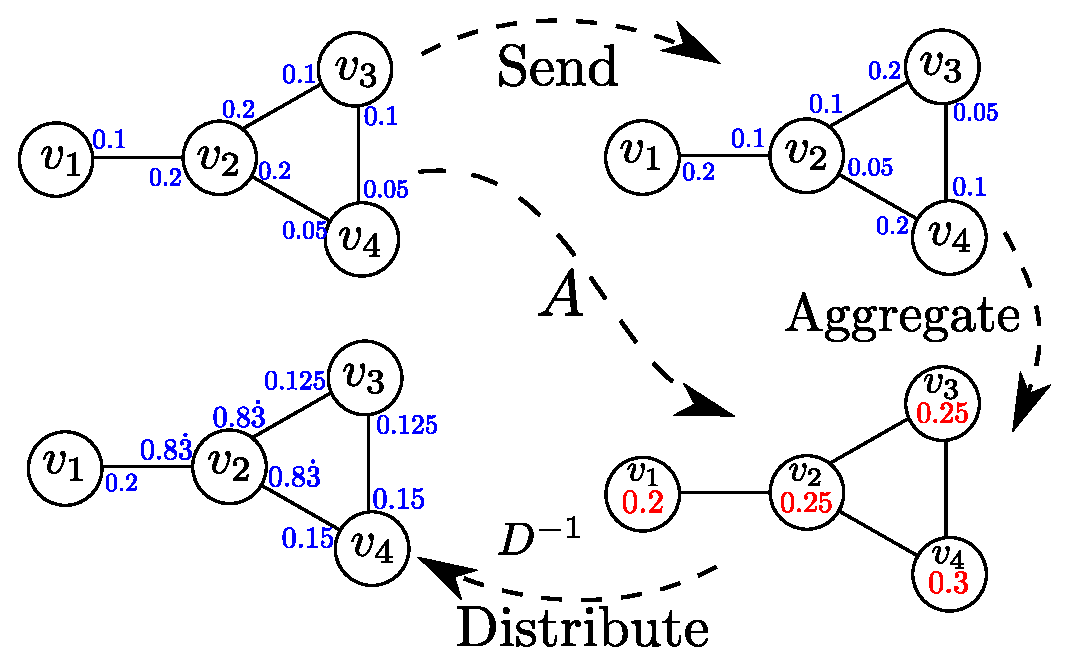
\includegraphics[scale=0.65]{WT.eps}
    \caption{The action of $W^T$ on the vector $x = ({\color{blue}0.1},{\color{blue}0.6},{\color{blue}0.2},{\color{blue}0.1})$.}
    \label{fig:Wt}
\end{figure}

\section{Hilbert Space Interpretation}
One can think of the $x$ vectors as living in the Hilbert space with inner product $\langle\cdot ,\cdot\rangle_D: \R^V \to \R$ given by:
\[
    \langle x,y \rangle_D = x^TDy
\]
And similarly the $p$ vectors live in the dual space with inner product: $\langle \cdot,\cdot\rangle_{D^{-1}}: \R^V \to \R$ given by:
\[
    \langle p,q \rangle_{D^{-1}} = p^TD^{-1}q
\]
for any $x$ the corresponding vector $p$ will equal $\Phi(x)$ where $\Phi$ is the isomorphism guaranteed by the Riesz representation theorem\footnote{Read more about it: \url{https://en.wikipedia.org/wiki/Riesz_representation_theorem}}.

\begin{figure}[h]
    \centering
 %   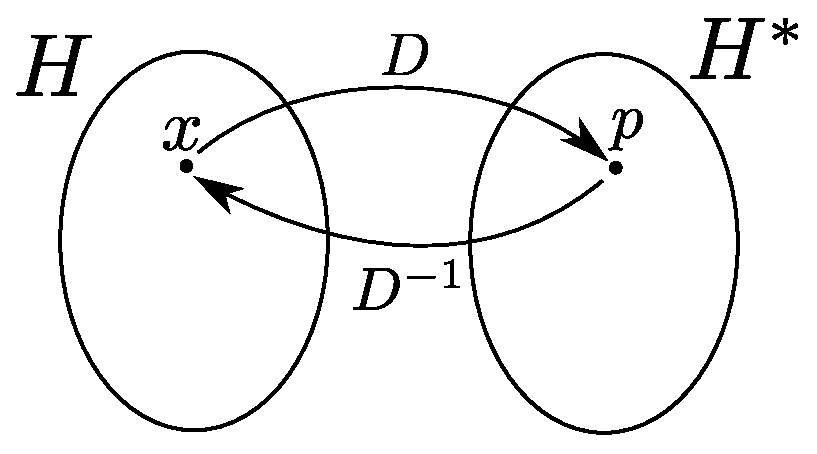
\includegraphics[scale=.75]{HSpaceSGT.eps}
    \caption{Vertex probability vectors $p$ live in the dual Hilbert space to that of edge mass vectors $x$.}
    \label{fig:my_label}
\end{figure}
\section{Measuring Convergence to the Fixed Point}
An important choice to make when tracking the dynamics of these processes, is the choice of potential function: how do we measure distance from the fixed point?\\

\noindent
In the \textbf{averaging process} it makes sense to track the distance of a mass assignment $x$ from the optimum by:
\[
    \phi_{avg}(x):= \sum_{i\in V} \pi_i \left(x_i - (\sum_{j \in V} \pi_j x_j)\right)^2 = Var_{i \sim \pi}(x_i)
\]

\noindent
By applying the conversion in $(\ref{change_of_basis})$ we see that this corresponds to:

\[
    \phi_{avg}(x) = ||x - \bar{x}||_{\pi}^2 = ||D^{-1}p - \bar{x} D^{-1}\vec{1} ||^2_D = ||p - \bar{x}\vec{1}||^2_{D^{-1}} = ||p-\pi||^2_{D^{-1}}
\]
which corresponds naturally to a way to measure distance from the optimum in the \textbf{random walk} process.

\section{Why Laplacians?}
The above analysis can provide motivation for the use of Laplacian matrices to study graph algorithms. One can in fact prove the following claim:
\begin{claim}
The potential function defined above is the quadratic form of the Laplacian of a suitably defined graph. I.e there exists some graph $H$ such that, for all $x \in \R^V$:
$\phi_{avg}(x) = x^TL(H)x$.
\end{claim}
\begin{proof}
One can define a graph $K_G$ as follows: $V(K_G) = V(G)= V$ and $E(K_G) = \binom{V}{2}$, so that the graph is complete, with weigths $w_{K_G}(ij) = \frac{d_id_j}{vol(G)}$~\footnote[1]{Recall that for any $S \subset V$: $vol(S):= \sum_{i \in S} d_i$ and $vol(G):= vol(V)$.}\\

\end{proof}

\noindent
We also observe that the value of the quadratic form $x^TL(G)x$ defined by the Laplacian matrix of $G$ measures the rate of convergence towards the stationary distribution at $x$. In fact, consider the continuous version of the averaging process given by:

\[
    \frac{dx(t)}{dt} = - (I-W^T)x(t)
\]


\noindent
We have:
\begin{align*}
    \frac{d}{dt}\left(||x - \bar{x}||_D^2\right) &= \left(\frac{d}{dt}x(t)\right)^TD(x(t)-\bar{x})\\
    &= \left(-(I-W^T)x(t)\right)^TD(x(t)-\bar{x})\\
    &= -x(t) (D-A)(x-\bar{x}) = -x^T(D-A)x
\end{align*}

\noindent
Where the last step above uses the fact that:
\[
    L\vec{1} = 0.
\]


% when \include is used, the extension should be avoided, otherwise the project won't compile the additional file.
\chapter{Positive Semidefinite Matrices}
In this chapter we will discuss positive semidefinite (PSD) matrices, a class of operators that plays and essential role both in spectral graph theory and in optimization as a whole.

\begin{definition}[PD/PSD Matrix]
A symmetric $n \times n$ matrix $M$ is said to be \emph{positive semidefinite} (PSD) if, for all vectors $x \in \R^n$ we have:
\[
    x^TMx \geq 0
\]
we denote this by $M \succeq 0$. Similarly, a symmetric $n \times n$ matrix $M$ is said to be \emph{positive definite} (PD) if, for all $x \in \R^{n}\setminus\{0\}$:
\[
    x^TMx > 0
\]
we denote this fact as $M \succ 0$.
\end{definition}

From the spectral theorem for symmetric matrices we get the following useful characterization of PSDness:

\begin{theorem}
A symmetric $n \times n$ matrix $M$ is PSD if and only if all of its eigenvalues are non-negative, and PD if they are strictly positive.
\end{theorem}
\begin{proof}
Every eigenvalue of $M$ arises as the value of $x^TMx$ for some $x \in \R^n$ (namely the corresponding normalized eigenvector) and hence if $M$ is PSD(/PD) then all eigenvalues must be non-negative(/strictly positive). On the other hand suppose that all the eigenvalues of $M$ are non-negative ($0 \leq \lambda_1 \leq ... \leq \lambda_n$) then we can write:
\[
    M = \sum_{i=1}^n \lambda_n v_iv_i^T
\]
where $v_1, ... , v_n$ is an orthonormal basis of eigenvectors of $M$. Hence, for every $x \in \R^n$:
\[
    x^TMx = \sum_{i=1}^n \lambda_n \langle v_i , x\rangle^2 \geq 0
\]
(similarly for PD matrices we get $>0$).
\end{proof}

We also state the following useful result without a proof:
\begin{theorem}[Sylvester's Criterion]
A matrix is PD if and only if all its leading principal minors are positive, and PSD if and only if all it's principal minors are non-negative.
\end{theorem}

We now prove a characterization of PSDness for matrices \footnote{from \href{https://people.eecs.berkeley.edu/~luca/bwca17/lectures/lecture04s.pdf}{Luca Trevisan's notes}} :
\begin{proposition}[Characterization of PSD Matrices]
A square matrix $M \in \R^{n\times n}$ is PSD (and hence symmetric) if and only if there exists vectors $x^{(1)}, ... , x^{(n)} \in \R^n$ such that $M_{i,j} = \langle x^{(i)}, x^{(j)} \rangle$.
\end{proposition}
\begin{proof}
Suppose that $x^{(1)}, ... , x^{(n)} \in \R^n$ exist as above, then clearly the matrix $M$ is symmetric and furthermore:
\[
    y^TMy = \sum_{i,j} y_i M_{ij}y_j = \left\langle \sum_i y_i x^{(i)}, \sum_j y_j x^{(j)}\right\rangle = \norm{\sum_iy_i x^{(i)}}^2 \geq 0
\]
so $M$ is PSD. Conversely we can use the spectral decomposition of $M$ to see that:
\[
    M = \sum_{k=1}^n\lambda_k v^{(k)}v^{{(k)}^T}
\]
giving that:
\[
    M_{ij} = \sum_{k=1}^n \lambda_k v_i^{(k)}v_j^{(k)}
\]
so that we can set:
\[
    x_k^{(i)} = \sqrt{\lambda_k}v^{(k)}_i
\]
and this satisfies the desired properties.
\end{proof}
Note the the above proposition goes hand in hand with the fact that any PSD matrix can be decomposed as $M = B^TB$. One example of such factorization is the Cholesky Decomposition / Cholesky Factorization, where $M$ is written as $LL^*$ for some lower-triangular matrix $L$. This exists for every hermitian PSD matrix, and when the matrix $M$ only has real entries, the matrix $L$ can also be chosen to only have real entry and the factorization becomes $M= LL^T$. If $M$ is PD then $L$ the Cholesky Factorization is unique, this is not necessarily true in the PSD case.\\

\begin{proposition}[PSD Matrices Form a Cone]
Let $A,B$ be $n\times n$ PSD matrices, we then have:
\begin{enumerate}
    \item $A+B \succeq 0$,
    \item if $\alpha \geq 0$ then $\alpha A \succeq 0$,
    \item if $\alpha,\beta \geq 0$  then $\alpha A + \beta B \succeq 0$.
\end{enumerate}
In particular, this means that the set of PSD matrices forms a cone.
\end{proposition}
\begin{proof}
We prove each of the above individually:
\begin{enumerate}
    \item For any $x \in \R^n$:
    \[
        x^T(A+B)x = x^TAx + x^TBx \geq 0.
    \]
    \item For any $x \in \R^n$:
    \[
        x^T(\alpha A) x = \alpha x^T A x \geq 0.
    \]
    \item Follows from the previous two parts.
\end{enumerate}
\end{proof}

We now introduce the matrix inner product:
\begin{definition}[Matrix Inner Product]
Given any two $n \times n$ matrices $A,B$ their (dot) inner product is the value:
\[
    A \bullet B := tr(A^TB) = \sum_{i,j} A_{i,j}B_{i,j}.
\]
\end{definition}
we now go on to prove that the one define above is, indeed, an inner product:
\begin{proposition}
The function $\bullet: \R^{n\times n}\times \R^{n\times n} \to \R$ defined above is a real inner product, i.e. satisfies:
\begin{description}
    \item[Symmetry] For any $A,B$ we have $A \bullet B = B \bullet A$,
    \item[Linearity] For any $A,B,C$ and $\alpha,\beta \in \R^n$ we have $(\alpha A+ \beta B) \bullet C = \alpha (A \bullet C) + \beta (B \bullet C)$,
    \item[Positive Definiteness] $A \bullet A \geq 0$ and $A \bullet A = 0 \iff A = 0$.
\end{description}
\end{proposition}
\begin{proof}
The inner product is clearly symmetric $(A^TB = (B^TA)^T$ so $A^TB$ and $B^TA$ have the same trace). For linearity one checks:

\begin{align}
    (\alpha A+ \beta B) \bullet C &= \sum_{i,j}(\alpha A_{i,j} + \beta B_{i,j})C_{i,j} = \alpha \sum_{i,j} A_{i,j} C_{i,j} + \beta \sum_{i,j} B_{i,j}C_{i,j} \\
    &= \alpha (A \bullet C) + \beta (B \bullet C)
\end{align}
Positive definitiness is also clear since $A \bullet A$ is a sum of squares.
\end{proof}

\begin{proposition}[Properties of the Matrix Inner Product]
Let $A$ and $B$ be symmetric matrices such that $A,B \succeq 0$ then $A \bullet B \geq 0$.
\end{proposition}
\begin{proof}
Using the spectral expansion of $A$:
\[
    A = \sum_{i=1}^n \lambda_iv_iv_i^T
\]
we have:
\[
    A \bullet B = tr\left(\sum_{i=1}^n \lambda_i v_iv_i^TB\right) = \sum_{i=1}^n\lambda_i tr\left(v_iv_i^TB\right) = \sum_{i=1}^n\lambda_i tr\left(v_iv_i^TB\right) = \sum_{i=1}^n\lambda_i tr\left(v_i^TBv_i\right) \geq 0
\]
\end{proof}




% ------------------------------------------ %
% ---------- End of Main Content  ---------- %
% ------------------------------------------ %

\iffalse

   The \appendix macro can be used to indicate that following
   sections or chapters are to be numbered as appendices.
   Appendices can be used for the article class too:

\fi

\appendix
\chapter{First Appendix}

\iffalse

   The backmatter behaves like the frontmatter.
   It has the same issue with section numbering.

\fi

\backmatter
\chapter{Last note}



\end{document}
